\documentclass{scrartcl}
\usepackage[utf8]{inputenc}
\usepackage[english]{babel} % Trennung nach der neuen deutschen Rechtschreibung
\usepackage[utf8]{inputenc}
\usepackage[T1]{fontenc}
\usepackage{lmodern}

\usepackage{amsmath} % Erweiterte Mathematik-Umgebung
\usepackage{amsfonts} % zusätzliche Mathematik-Schrifttypen (v.a. \mathbb für Mengen)
\usepackage{ulem}

\usepackage{graphics}%soll beim Graphiken einfügen hilfreich sein
\usepackage{graphicx}
\usepackage{wrapfig}%lässt Textumflossene Bildeinbindung zu
\usepackage{epstopdf}%soll eps in pdf umwandeln

\usepackage[a4paper, portrait, margin=2.5cm]{geometry}

\titlehead{\centering University of Luxemburg}
\subject{Travaux Pratiques}
\title{Law of Van der Waals}
\subtitle{Joana Ferreira}
\date{TP Session 5/11/2021}
\author{Louis-Hendrik Barboutie (020157041C)\\ Frederik Ehl (0201719742) \\ Florence Schmerber (0201845640)}

\begin{document}

\maketitle

\clearpage

\tableofcontents
\listoffigures
	
\clearpage

\section{Introduction}

The aim of this experiment is to use and understand two important equation in thermodynamics: the van der Waals equation and the equation of Clausius-Clapeyron. The van der Waals equation gives us a relation between the volume $V$ the pressure $p$, the temperature $T$ and the amount of mole $n$.

\begin{equation}
    (p + \frac{a}{V_m^2})(V_m-b)=RT\nonumber
\end{equation}

On the other hand, the Clausius-Clapeyron equation gives us the relation between the pressure $p$ at a constant volume and the temperature $T$, with $L$ being the heat of evaporation, which is temperature dependent.

\begin{equation}
    \frac{dp_V}{dT} \approx \frac{L}{T(V_g-V_l)}\nonumber
\end{equation}

\section{Theoretical Discussion}

\subsection{Ideal gas law}

The starting point of this TP, the ideal gas law, states:

\begin{equation}
    \boxed{pV=nRT}
\end{equation}

It gives us a relation between the volume V ($m^3$), the pressure p (Pa), the temperature (K) and the ideal gas constant $R=8,314J\cdot mol^{-1}\cdot K^{-1}$ and n the number of molecules (mol) of the gas.

\subsection{Law of Van der Waals}

The experience shows that real gases show the following properties:

\begin{itemize}
    \item The compressibility is finite.
    \item They can be liquidated if their temperature is sufficiently low.
    \item There can be a coexistance of two phases: liquid and gas.
\end{itemize}

However, this equation does not describe the behaviour of real gases very well, and although we can use it as a first approximation, we will introduce some corrections:

\medskip

Firstly, we need to take into account the co-volume of the gas molecules (the volume which is occupied by the molecules themselves), which is subtracted from the total available volume. Called the \textit{excluded volume}, it is denoted with $b$. If we approximate the molecules as spheres, then $b = 4 V_p$, where $V_p$ is the proper volume of the molecules.

\medskip

Secondly, the pressure is adjusted to take the interaction forces between molecules into account, by introducing the internal pressure $p_{internal} = \frac{a}{V_m^2}$, and adding it to the total pressure.

\medskip

By including these corrections in the ideal gas law, we finally obtain the Van der Waals equation:

\begin{equation}
    \boxed{(p + \frac{a}{V_m^2})(V_m-b)=RT}
\end{equation}

Which we can rewrite for $n$ moles gas:

\begin{equation}
    \boxed{(p + \frac{n^2a}{V^2})(V-nb)=nRT}
\end{equation}

Note that for low pressures and high temperatures, this equation reduces to the ideal gas law. 

\subsection{p(V) diagrams}

When studying the properties of a gas, we can vary three main factors: pressure, volume and temperature. Ideally we want to observe the changes when only one changes and the other two parameters are held constant. We can do so in a p(V) diagram. It is a plot of the pressure as function of volume, where one has to detail the temperature at which the data has been acquired.
A transformation of the system at constant pressure is called \textit{isobar}, at constant volume \textit{isochor} and at constant temperature \textit{isothermal}.

\begin{figure}[h]
   \centering
    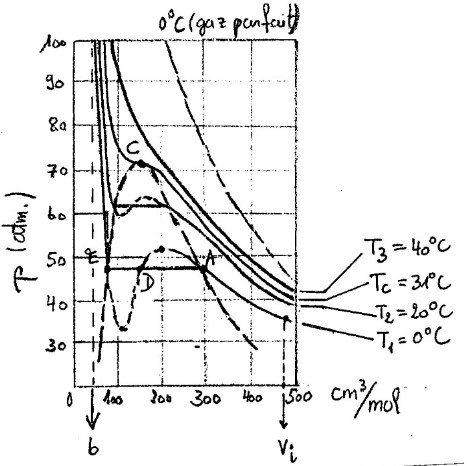
\includegraphics[width=7cm]{pvDiagramExample.jpg}
    \caption{pV diagram with isothermals of a real gas}
    \label{fig:1}
\end{figure}

While the Van der Waals equation is a much more precise representation of real gases, it isn't entirely accurate. Most notably, it is unable to describe the behaviour of a real gas in the so-called \textit{coexistence region}. 
This is a set of pressure, temperature and volume ranges, where both liquid and gaseous states coexist. This phenomenon can be observed: when in this region, the pressure of the element does not vary, despite varying the volume, at a set temperature.

\medskip 

Each gas has a proper coexistence region, and an associated \textit{critical temperature} $T_C$ and the \textit{critical pressure} $p_C$. When reaching this critical point, one can observe the phenomenon of \textit{critical opalescence}, where gas and liquid cannot be distinguished from each other. Coexistence of both states can only be observed if we make measurement at temperatures $T < T_C$. If $T > T_C$ however, we do not observe a constant pressure evolution. This will help us in determining the critical temperature and pressure. 

\section{Experimental setup}

A tube is filled with gaseous SF6 (sulfur hexafluoride) and surrounded by water. During the experiment we will vary the temperature of the surrounding water, which will in turn transfer heat to the gas and thus give us the ability to control the temperature of the gas. A thermometer submerged in the water gives readings of its temperature. The tube is also partially filled with liquid mercury, of which the quantity can be adjusted by turning a wheel attached to the apparatus. We can vary the amount of mercury and thereby modify the available volume for the gas inside the tube. The pressure inside the tube is measured via a barometer, whose detector is inside the tube.

\begin{figure}[htbp]
    \centering
    \includegraphics[width=12cm]{1636213691539.jpg}
    \caption{Experimental Setup}
    \label{fig:2}
\end{figure}

\section{Procedure}

\subsection{Determination of the van der Waals coefficients for SF6}

The main goal of this part of the experiment is to plot the isothermals for 10 different temperatures between 13°C and 55°C . During the experiment we take readings of the pressure for different volumes in steps of approximately $0.3mL$ or $0.2mL$, at constant temperature. This allows us to plot the isothermals of the pressure as a function of the volume.

\medskip

\textit{Remark: It wasn't really possible to write down the values from start to finish at a constant temperature for lower temperature (under 25 °C). During the experiment the temperature would inevitably go up. To counterbalance this, we considered the temperature of our isothermal to be the average of the temperature of the gas from the beginning to end of readings.}

\medskip

Then we want to approximate the number of mole in the gas. In order to do that, we consider the isothermal of the highest temperature, in our case $T = 55^{\circ}C$, which has the closest to resemblance to the ideal gas law. We then make a fit using the ideal gas equation $pV=nRT$, which we can rearrange into $p =  \frac{nRT}{V}$. We get an inverse relationship between $p$ and $V$. 

\section{Results}

\subsection{Determination of the van der Waals coefficients for SF6}
We obtained the following graph of the pressure as a function of the volume, which corresponds to the isothermals for each temperature.

\begin{figure}[h]
    \centering
    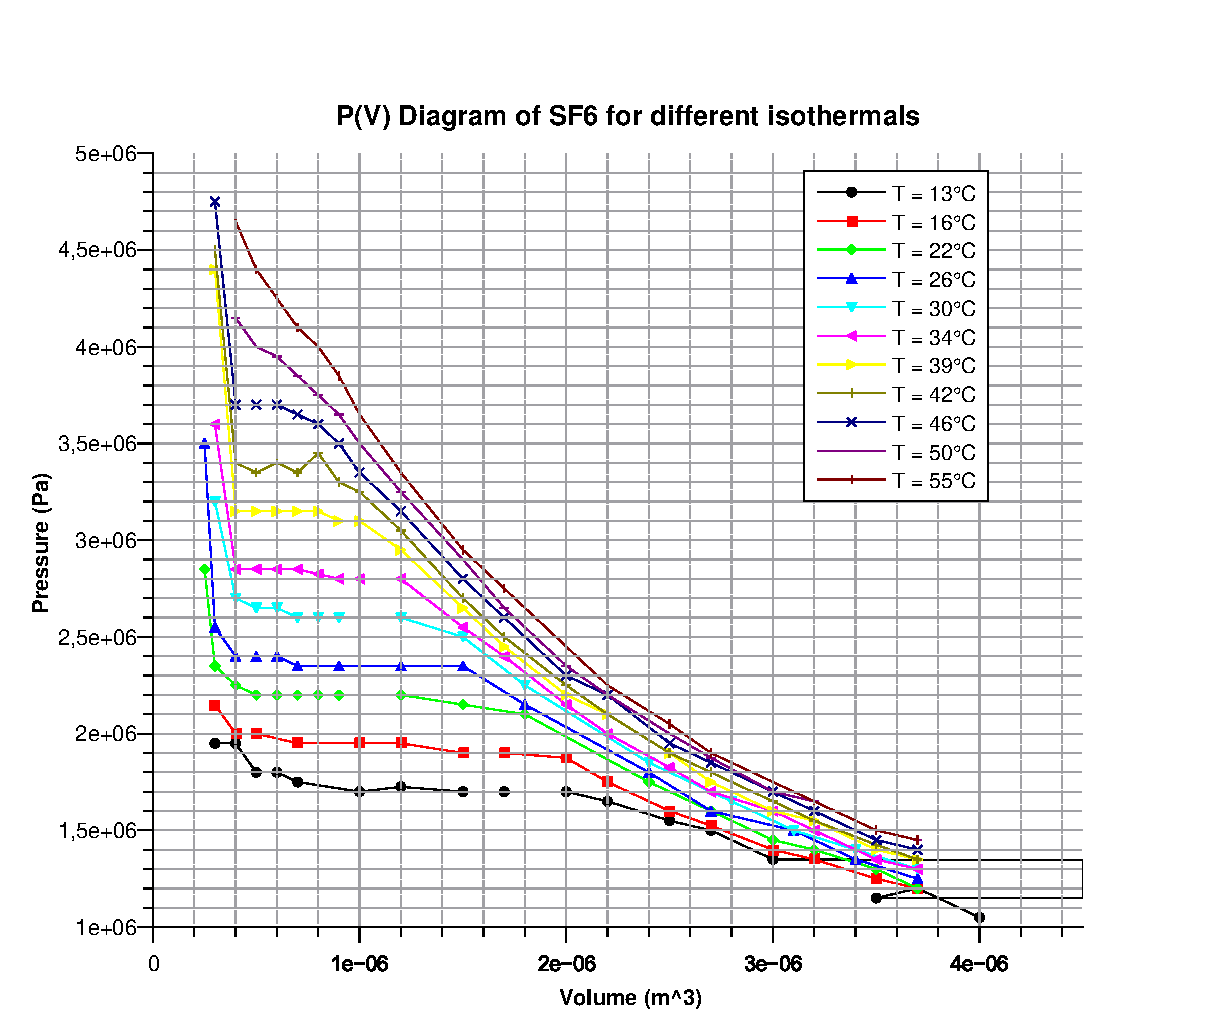
\includegraphics[width=12cm]{PVDiagramSF6.eps}
    \caption{P(V) diagram of SF6}
    \label{fig:3}
\end{figure}

We could observe the coexistence state of the element, when the element is both a liquid and a gas at temperature approximately below 46 °C.

\medskip

Next we want to determine the amount of gas in the tube. Using the highest isothermal, and the built-in fitting wizard of qtiPlot we obtain $\boxed{n \approx 9,96 \cdot 10^{-4} mol}$.

\begin{figure}[h]
    \centering
    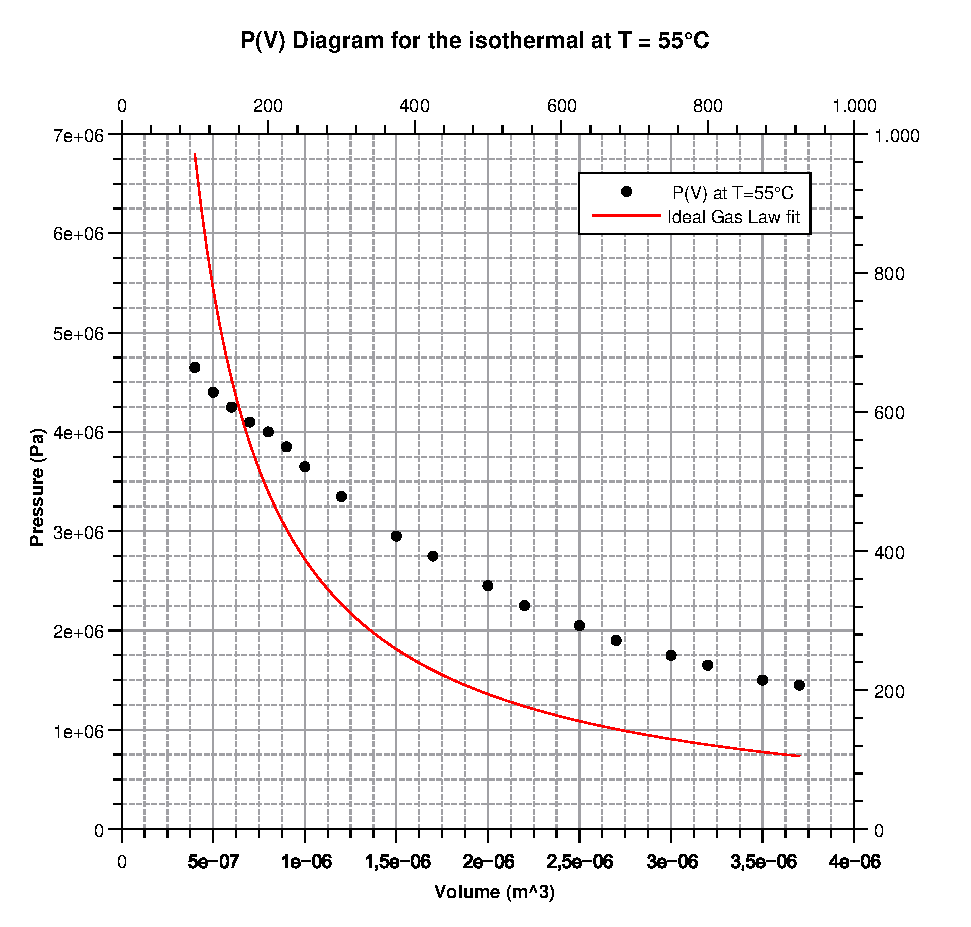
\includegraphics[width=6.5cm]{IdealGasLawFitTemp55C.eps}
    \caption{Ideal gas law fit to the highest isothermal}
    \label{fig:5}
\end{figure}

\newpage

%we use the highest temperature because it is closer to an ideal gas, because there is no coexisting of gas and liquid
From the figure 3 we can estimate the critical temperature $T_c$ and the critical pressure $p_c$. We guesstimate $\boxed{T_C = 48^{\circ}C}$ and $\boxed{p_C = 3,85 \cdot 10^6 Pa}$.

We can now calculate the values of a and b (see section 2.2):
We know that:
\begin{equation} \nonumber
    \begin{cases}
    p_C = \frac{a}{27b^2} \\
    T_C = \frac{8a}{27Rb}
    \end{cases}
\end{equation}

We can solve for a and b:
\begin{equation} \nonumber
    \begin{cases}
    a = p_C27b^2 \\
    b = \frac{8a}{27RT_C}
    \end{cases}
    \Leftrightarrow
    \begin{cases}
        a = \frac{27R^2T_C^2}{64p_C} \\
        b = \frac{RT_C}{8p_C}
    \end{cases}
\end{equation}

We find \boxed{a = 6.99 \cdot 10^-1 \ Pa \cdot  m^6 \cdot mol^{-2}} \ and \  \boxed{b = 8,67 \cdot 10^{-5} \ m^3 \cdot mol^{-1}}

\subsection{Representation of the van der Waals equation}

Now that we have approximated values for each coefficient of the van der Waals equation a, b and n, we can plot the van der Walls equation for each isothermal (see Appendix). In order to do that, we rearrange the van der Waals equation to solve for $p$: $p =  \frac{nRT}{V-nb}-\frac{n^2a}{V^2}$ and plot it in qtiPlot where we use the approximated values for a, b and n (not held constant).
Because the equation doesn't describe the coexistence region, we will simply disregard the values where the pressure stays constant. When averaging the values we get for each fit, we can obtain a much more accurate value for a, b and n. We get:

\medskip
\centering
\begin{tabular}{|c|c|c|c|}
    \hline
     Temperature (in °C) & a (in $Pa \cdot m^6 \cdot mol^{-2}$) & b (in  $m^3 \cdot mol^{-1}$) & n ( in $mol$) \\
     \hline
     13 & $ 0,823 $ &$ 9,28 \cdot 10^{-5} $ & $ 1,81 \cdot10^{-3} $ \\
     \hline
     16 & $ 0.709 $ & $ 7,84 \cdot 10^{-5} $ & $ 2,02 \cdot 10^{-3} $  \\
     \hline
     22 & $ 2,9 \cdot 10^{-2}$ & $ 3,46 \cdot 10^{-6}$ & $ 9,2 \cdot 10^{-5} $ \\
     \hline
     26 & $ 2,74 \cdot 10^{-2}$ & $ 3,19 \cdot 10^{-6}$ & $8,7 \cdot 10^{-5} $\\
     \hline
     30 & $ 0,714 $ & $ 7,7 \cdot 10^{-5} $ & $ 2,04 \cdot10^{-3} $ \\
     \hline
     34 & $ 7,82 \cdot 10^{-3} $ & $ 8,7 \cdot 10^{-7} $ & $ 2,85 \cdot 10^{-5}$ \\
     \hline
     39 & $ 0,725 $ & $ 7,8 \cdot 10^{-5} $ & $ 2,08 \cdot 10^{-3} $\\
     \hline
     42 & $ 0,918 $ & $ 8,611 \cdot 10^{-5} $ & $ 2,05 \cdot 10^{-3} $\\
     \hline
     46 & $ 0,712 $ & $ 7,61 \cdot 10^{-5} $ & $ 2,1 \cdot 10^{-3}$\\
     \hline
     50 & $ 0,76 $ & $ 8,299 \cdot 10^{-5} $ & $ 2,20\cdot 10^{-3} $\\
     \hline
     55 & $ 0,74 $ & $ 8,17 \cdot 10^{-5} $ & $ 2,20 \cdot10^{-3} $ \\
     \hline
\end{tabular}
\flushleft
we get the following average values of a,b and n:

\begin{equation}
    \boxed{a_{avg} = 6,01 \cdot 10^{-5} \ Pa \cdot m^6 \cdot mol^{-2}} \hspace{1cm}
    \boxed{b_{avg}=6,004 \cdot 10^{-5} \ m^3 \cdot mol^{-1}} \hspace{1cm} \boxed{n_{avg}= 1,5 \cdot 10^{-3} \ mol } \nonumber
\end{equation}

\subsection{Determination of the latent heat }

In the coexistence region, as we can see on figure 4, the pressure doesn't depend on the volume, but on the temperature. Because of this dependency we can use the Clausius-Clapeyron equation. For this part we want to plot the vapour pressure curve and find the latent heat of vaporization. 
First, we choose a volume, where you can observe the coexistence region, in our case we choose $0,5 ml$. Then with values of this exact volume, we plot the pressure as a function of the inverse temperature $1/T$ (see figure 6). Using the wizard fit on qtiplot, and plotting the fit for $A \cdot e^{\frac{-L}{RT}}$ we get immediately the value for $\boxed {L= 16,62 \ kJ.mol^-1}$

\begin{figure}[ht]
    \centering
    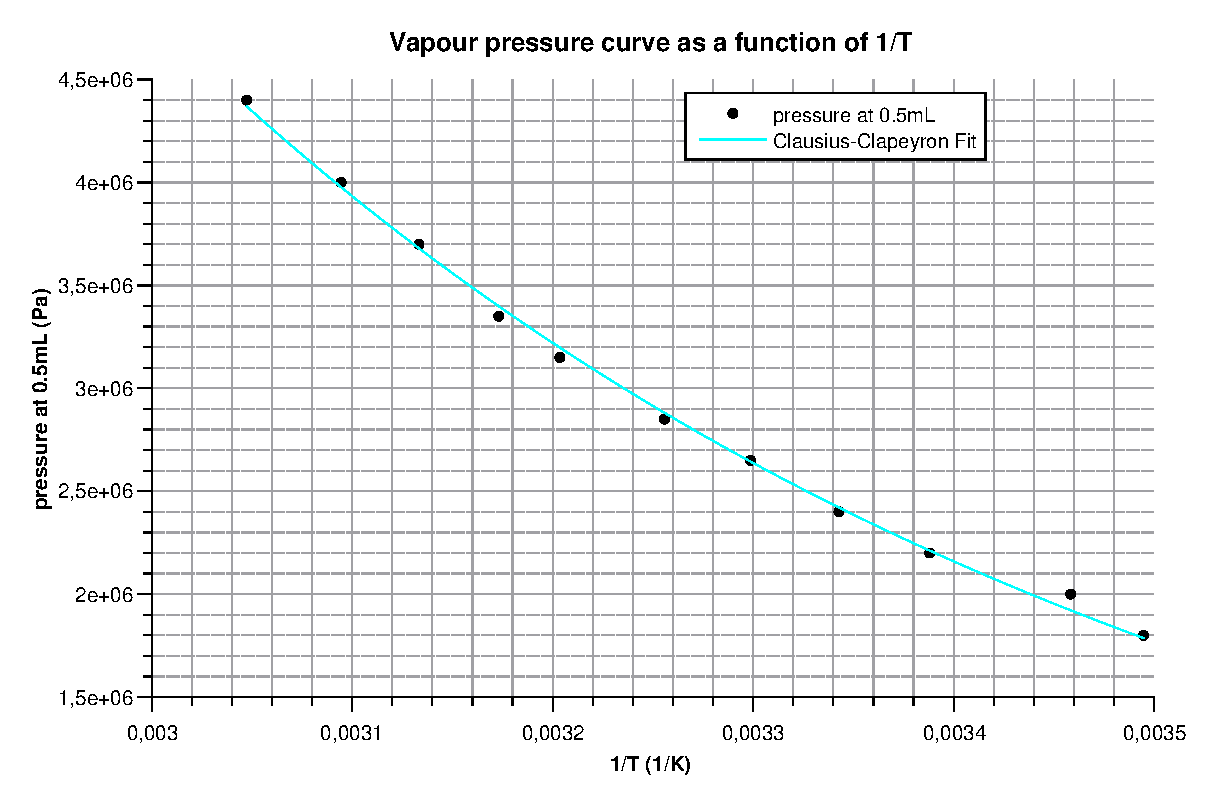
\includegraphics[width=12cm]{ClausiusClapeyronFit.eps}
    \caption{Vapour pressure as a function of 1/T}
    \label{fig:6}
\end{figure}

\newpage

\section{Conclusion}

During this series of experiments we determined some properties of $SF_6$ by making use of the Van der Waals equation and the Clausius-Clapeyron equation. Most notably, we determined the covolume, the internal pressure, the amount of moles and the latent heat of vaporization of sulfur hexafluoride  , by plotting the isothermals for each temperature.
We assume the results to be satisfying, although not very accurate. We did our best to get the most precision, by taking many readings, thus minimizing our error. However the inaccuracies origin from the reading method itself, the inability to conserve constant temperature accurately, get precise pressure readings, or change the volume with high precision. Also, the fact that we had to use three parameters to plot the curve reduced the accuracy of the result.%To improve the accuracy of the experiment one would have to take more measurements, also for lower temperatures.  

\section{Appendix}

\subsection{Determination of $p_c$, $T_c$ and $V_{CM}$}

At the critical point of a substance, there exists a coexistence of gas and liquid, which means it has a critical temperature $T_c$, a critical pressure $p_c$ and a critical volume $V_{CM}$. The isothermal at that point C is characterized by a horizontal tangent, which is also an infliction point.
This is the case when:

\begin{equation}
    \frac{\partial p}{\partial V} = 0 \hspace{1cm} \frac{\partial^2 p}{\partial V^2}=0
\end{equation}

To determine $p_c$, $T_c$ and $V_{CM}$ we have to use the \textit{Van der Waals equation} for one mole:

\begin{equation}
    p=\frac{RT}{V-b}-\frac{a}{V^2}
\end{equation}

Now we calculate the first derivative of p:

\begin{align}
\frac{\partial p}{\partial V} = 0 =\frac{-RT}{(V_{CM}-b)^2}+\frac{2a}{V_{CM}^3}\nonumber
\end{align}
\begin{equation} 
\begin{split}
\frac{2a}{V_{CM}^3}=\frac{RT}{(V_{CM}^2-b)^2}
\end{split}
\end{equation}

 And the second derivative:
 
\begin{align}
\frac{\partial^2 p}{\partial V^2}=0=\frac{2RT}{(V_{CM}-b)^3}-\frac{6a}{V_{CM}^4}\nonumber
\end{align}
\begin{equation} 
\begin{split}
 \frac{6a}{V_{CM}^4}=\frac{2RT}{(V_{CM}-b)^3}
\end{split}
\end{equation}

When we divide $\frac{\partial p}{\partial V}$ (equation 3) by $\frac{\partial^2 p}{\partial V^2}$ (equation 4) we get:

\begin{align}
\frac{\frac{2a}{V_{CM}^3}}{\frac{6a}{V_{CM}^4}} = \frac{\frac{RT}{(V_{CM}-b)^2}}{\frac{2RT}{(V_{CM}-b)^3}}\nonumber
\end{align}
\begin{equation} 
\begin{split}
\frac{V_{CM}}{3}=\frac{V_{CM}-b}{2}
\end{split}
\end{equation}

If we solve this equation we get $\boxed{V_{CM}=3b}$
\newline

We can now plug $V_{CM}$ into equation 3:

\begin{equation}
    \frac{2a}{27b^3} = \frac{RT_c}{(3b-b)^2}
\end{equation}

When we solve this equation we get $\boxed{T_c= \frac{8a}{27Rb}}$
\newline

To get the value for $p_c$ we simply take the van der Waals equation again and plug in the values of $T_c$ and $V_{CM}$:

\begin{align}
 p_c= \frac{R\frac{8a}{27Rb}}{2b}-\frac{a}{9b^2}\nonumber
\end{align}
\begin{equation} 
\begin{split}
p_c=\frac{4a}{27b^2}-\frac{a}{9b^2}
\end{split}
\end{equation}

Which gives us $\boxed{p_c=\frac{a}{27b^2}}$

\subsection{Van der Waals equation for isothermals}

\begin{figure}[htbp]
  \centering
  \begin{minipage}[b]{0.4\textwidth}
    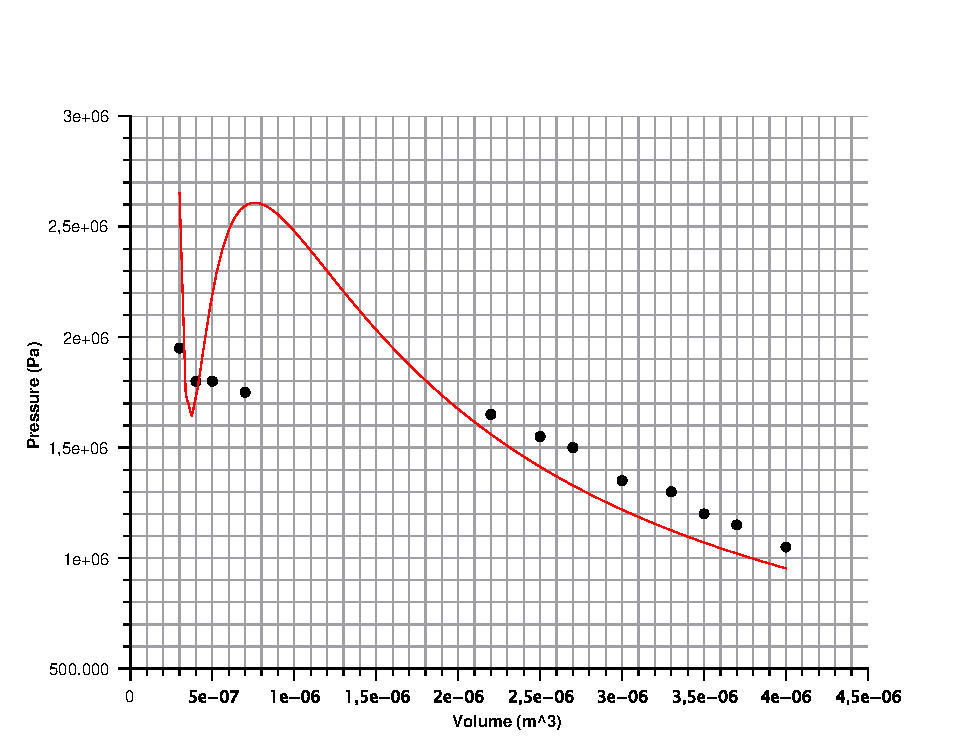
\includegraphics[width=\textwidth]{VdW13C.eps}
    \caption{13°C}
  \end{minipage}
  \hfill
  \begin{minipage}[b]{0.4\textwidth}
    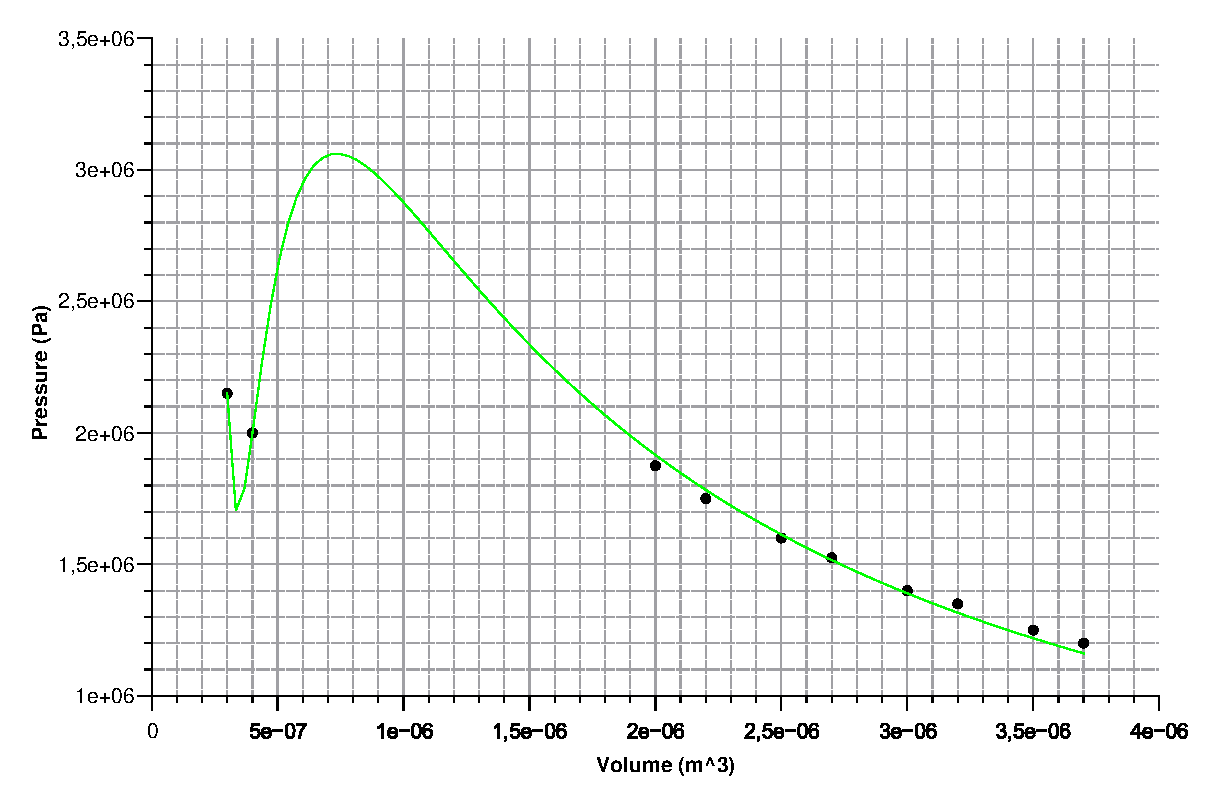
\includegraphics[width=\textwidth]{vdw16.eps}
    \caption{16 °C}
  \end{minipage}
\end{figure}

\begin{figure}[htbp]
  \centering
  \begin{minipage}[b]{0.4\textwidth}
    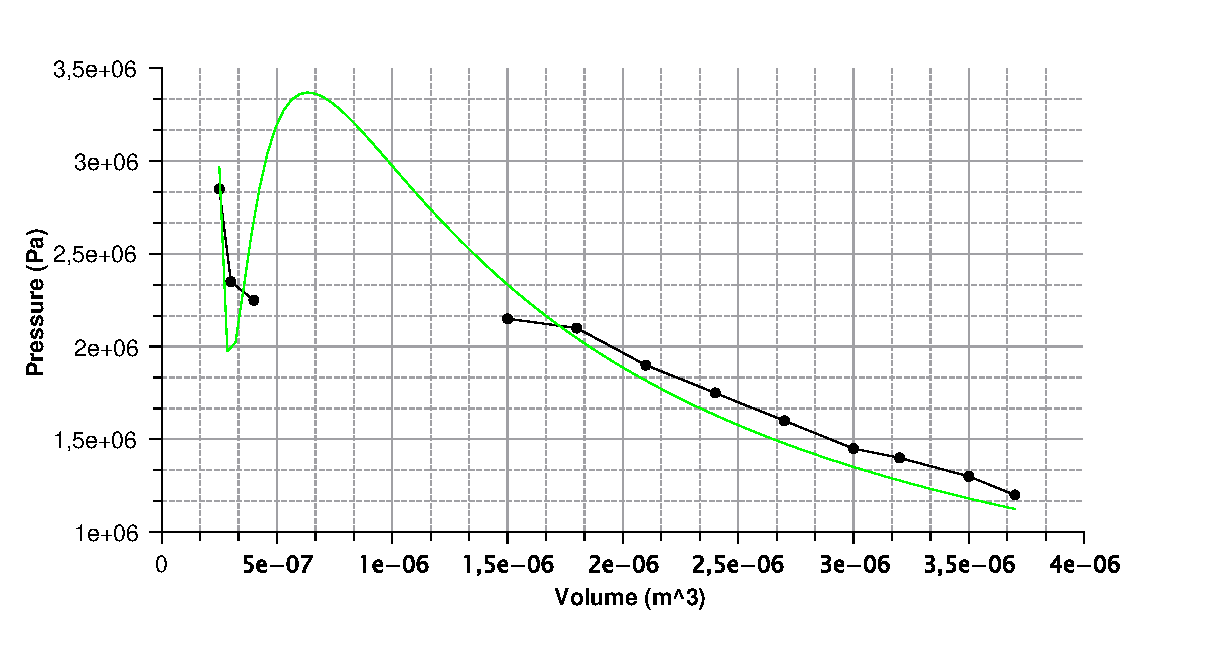
\includegraphics[width=\textwidth]{vdw22.eps}
    \caption{22 °C}
  \end{minipage}
  \hfill
  \begin{minipage}[b]{0.4\textwidth}
    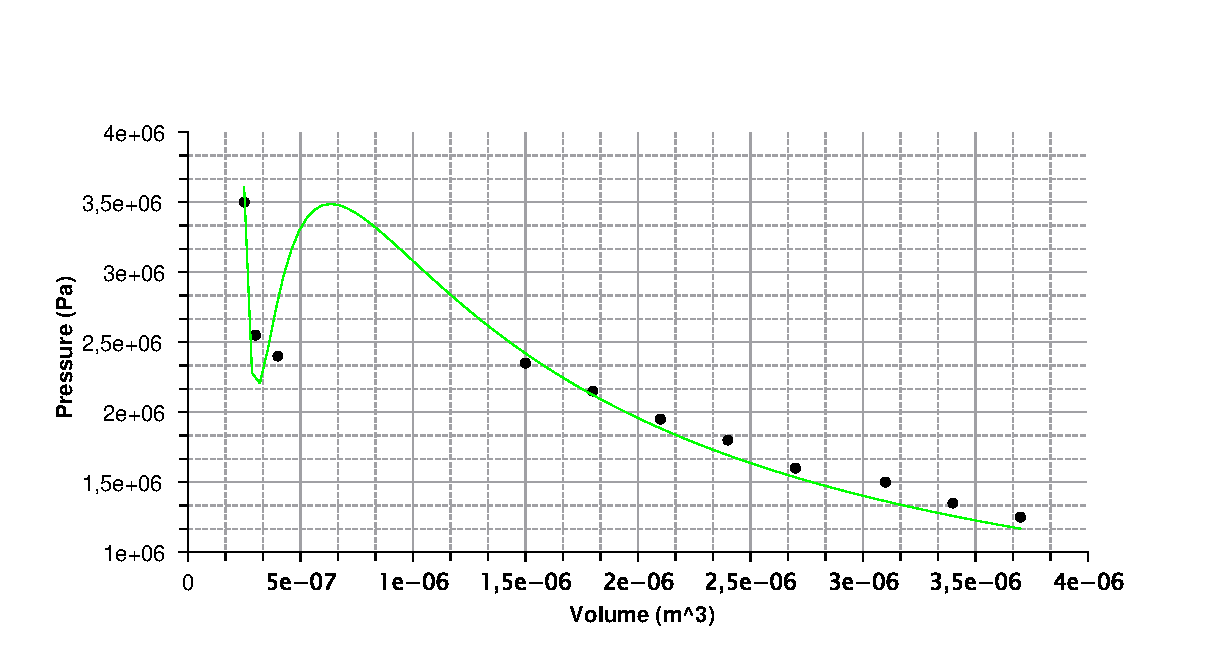
\includegraphics[width=\textwidth]{vdw26.eps}
    \caption{26 °C}
  \end{minipage}
\end{figure}

\begin{figure}[!tbp]
  \centering
  \begin{minipage}[b]{0.4\textwidth}
    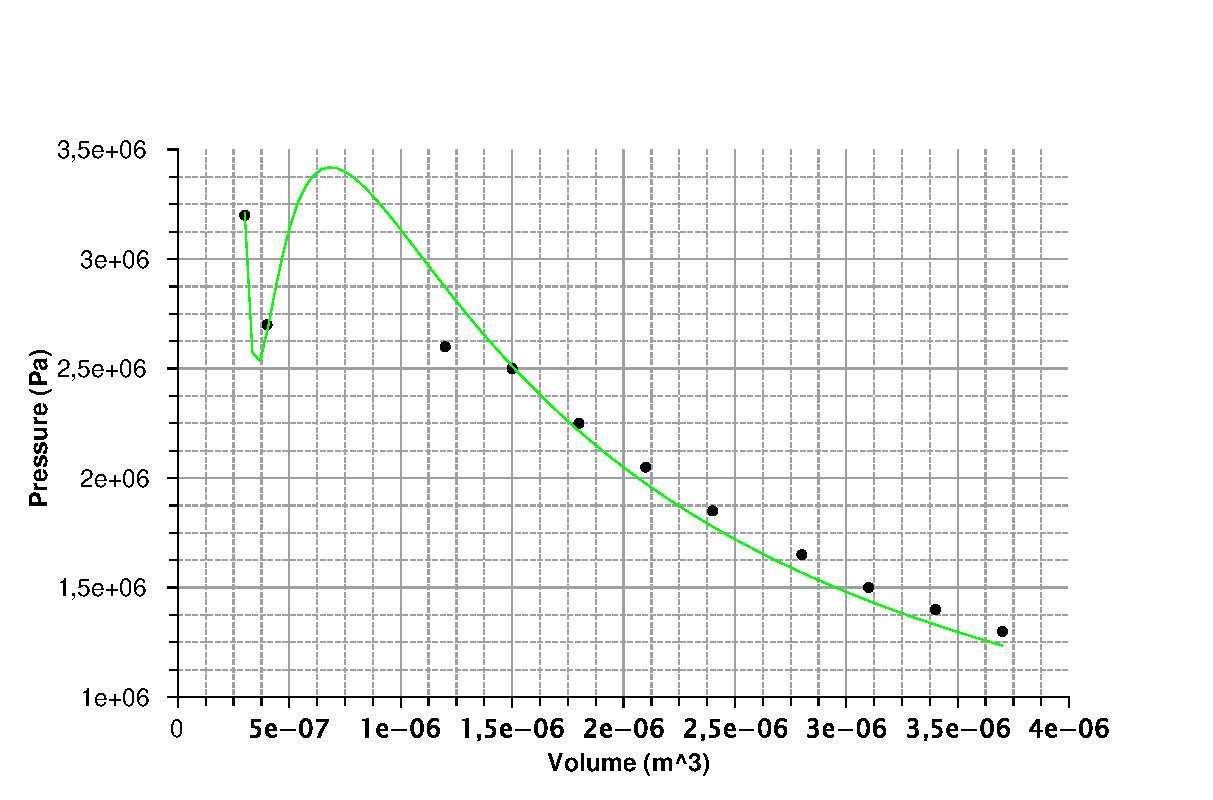
\includegraphics[width=\textwidth]{vdw30.eps}
    \caption{30 °C}
  \end{minipage}
  \hfill
  \begin{minipage}[b]{0.4\textwidth}
    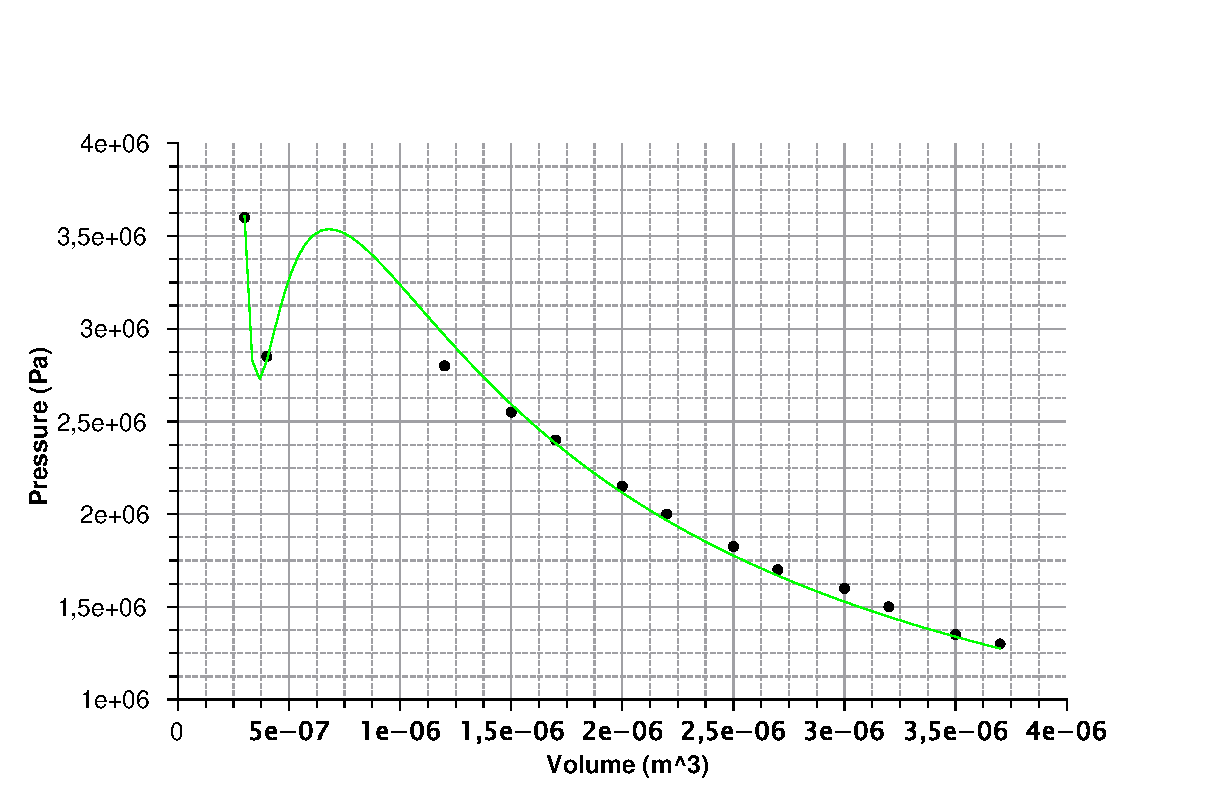
\includegraphics[width=\textwidth]{vdw34.eps}
    \caption{34 °C}
  \end{minipage}
\end{figure}

\begin{figure}[!tbp]
  \centering
  \begin{minipage}[b]{0.4\textwidth}
    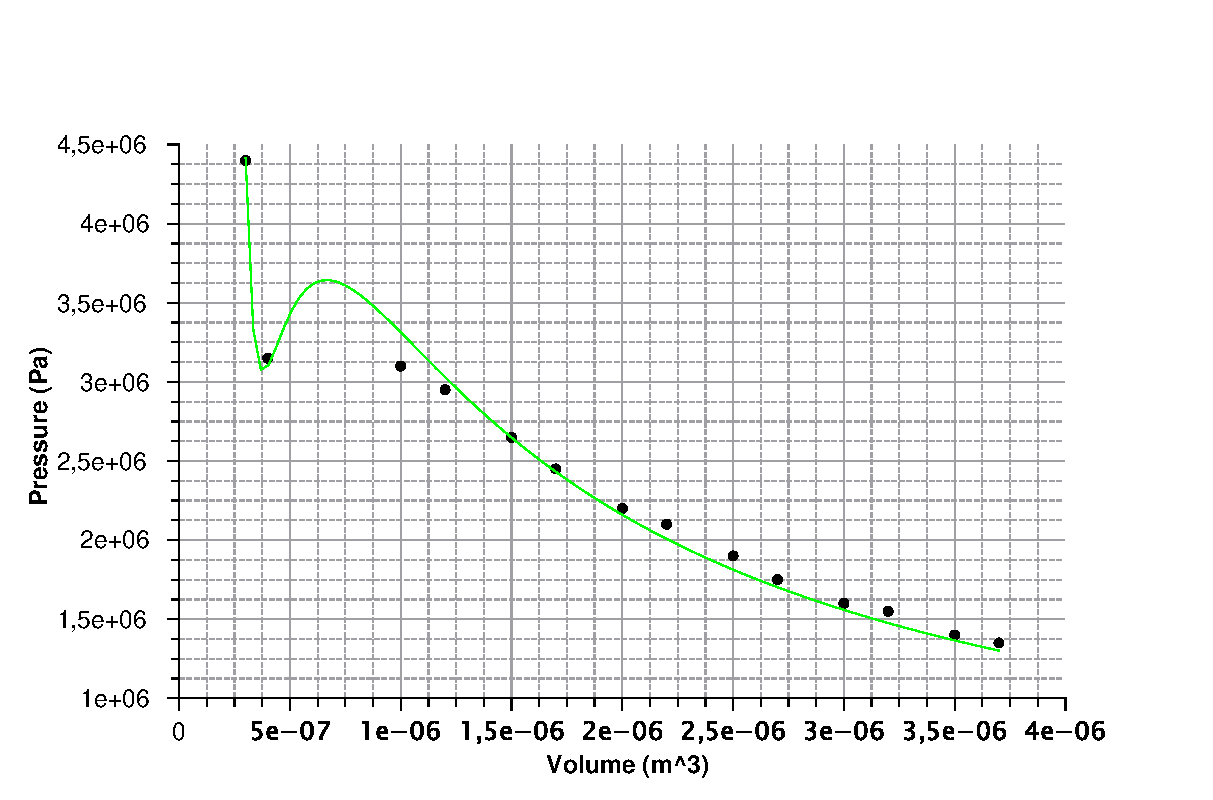
\includegraphics[width=\textwidth]{vdw39.eps}
    \caption{39 °C}
  \end{minipage}
  \hfill
  \begin{minipage}[b]{0.4\textwidth}
    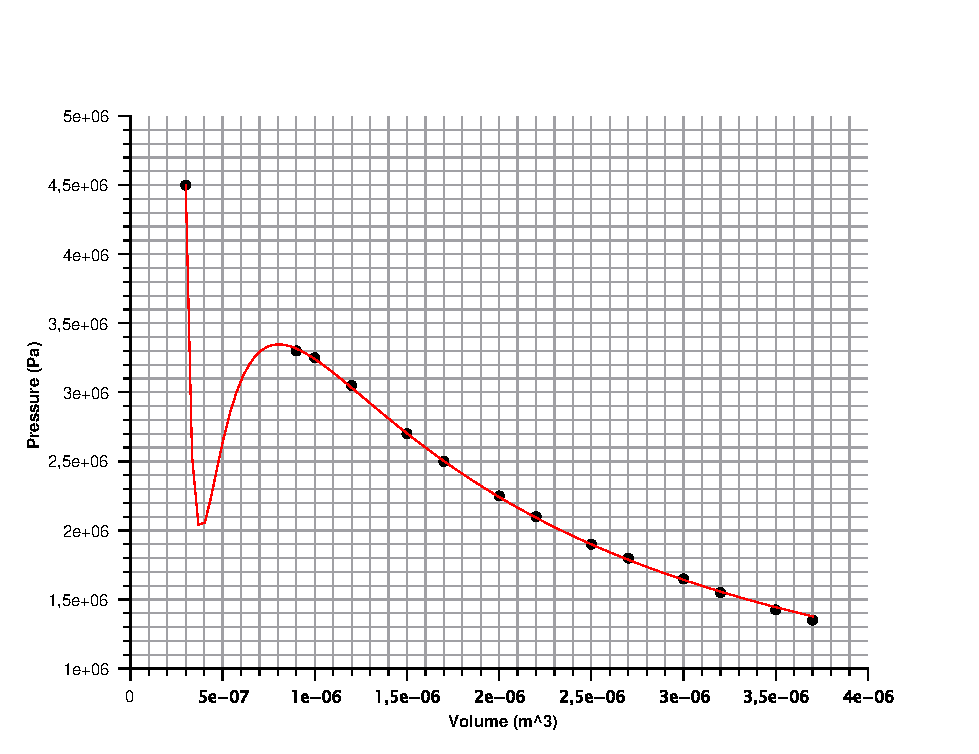
\includegraphics[width=\textwidth]{VdW42C.eps}
    \caption{46 °C.}
  \end{minipage}
\end{figure}

\begin{figure}[!tbp]
  \centering
  \begin{minipage}[b]{0.4\textwidth}
    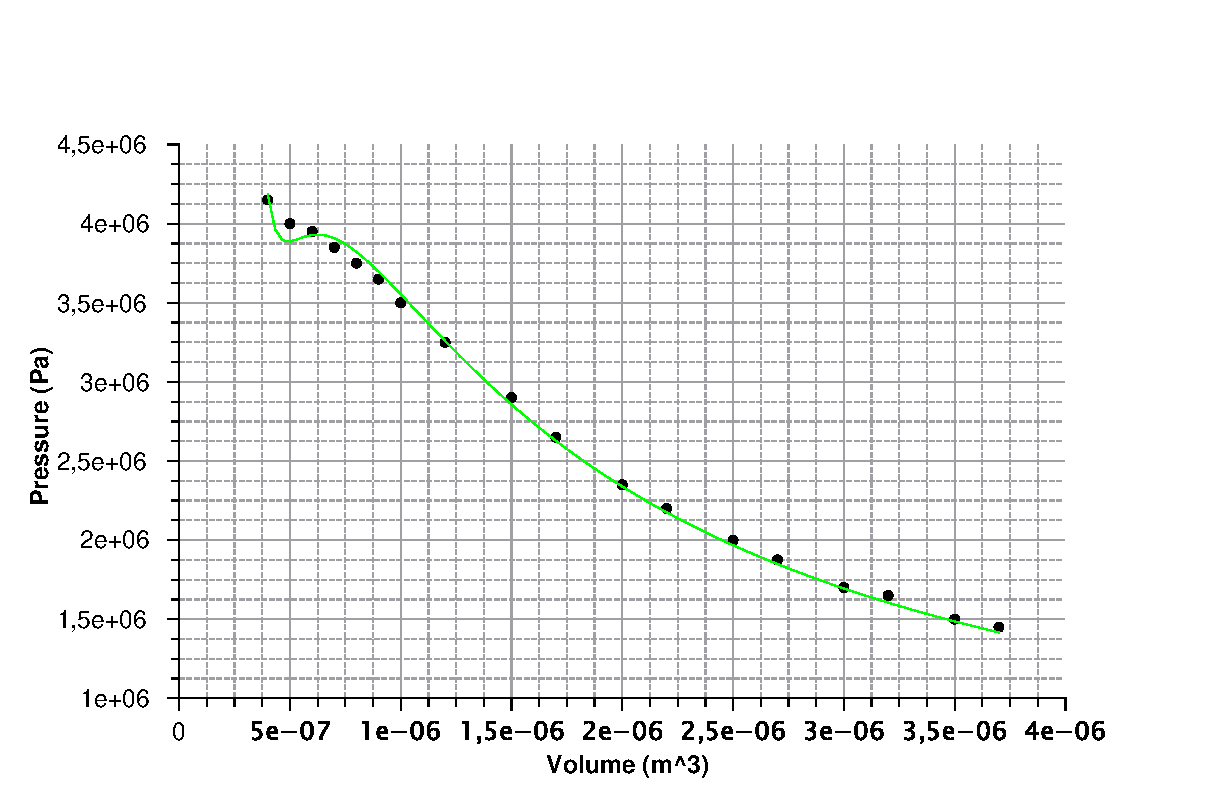
\includegraphics[width=\textwidth]{vdw50.eps}
    \caption{50 °C}
  \end{minipage}
  \hfill
  \begin{minipage}[b]{0.4\textwidth}
    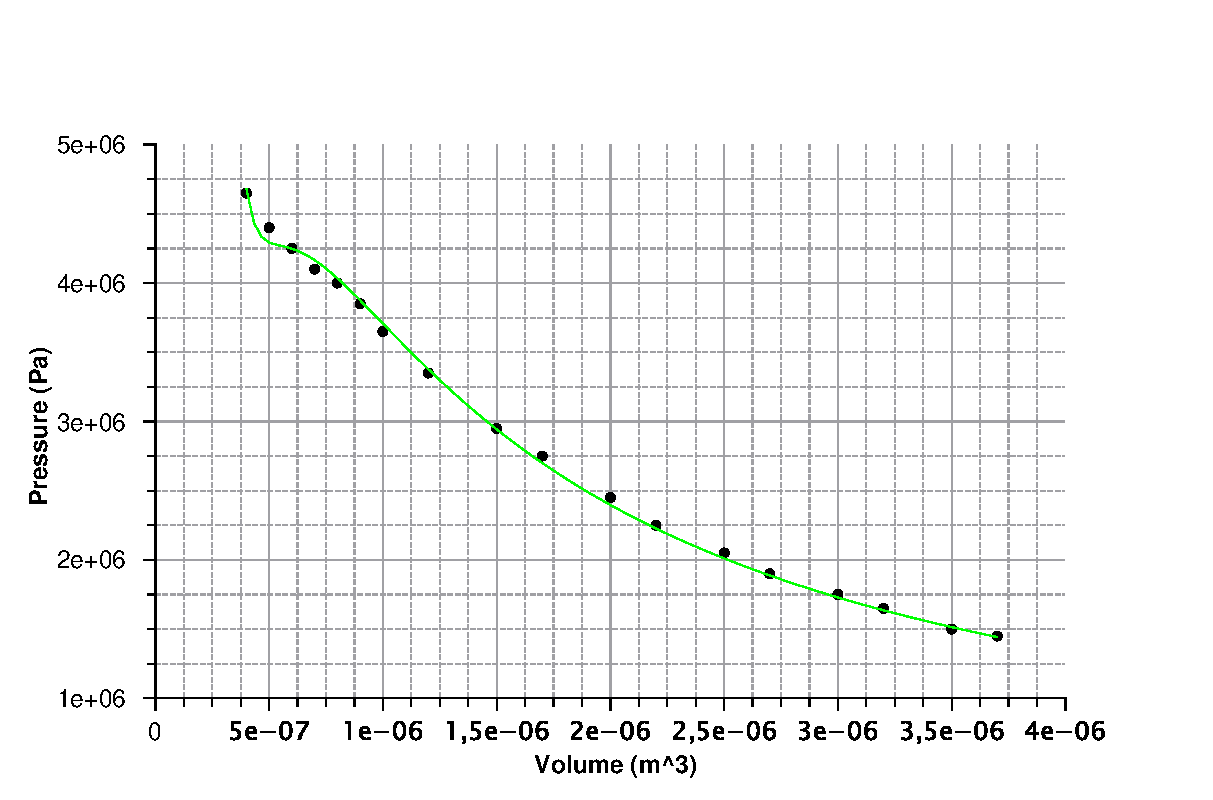
\includegraphics[width=\textwidth]{vdw55.eps}
    \caption{55 °C}
  \end{minipage}
\end{figure}

\end{document}